% Chapter Template

\chapter{Two-stage Classification Method for Automatic Reading Comprehension } % Main chapter title

\label{Chapter3} % Change X to a consecutive number; for referencing this chapter elsewhere, use \ref{ChapterX}

\section{Introduction}

Teaching reading comprehension in an online learning environment is challenging to instructors who need to provide learners with reading material that is authentic, thematically diverse, and reader level appropriate. The system we developed in the previous chapter helps language instructors detect the grammatical difficulties of reading materials found online, but it still does not help eliminate the efforts they need to expend on developing practice exercises and quizzes. In order for second and foreign language learners to master a difficult skill like reading comprehension, they need a great deal of practice, which means more training exercises need to be prepared. To solve this problem,  this chapter presents a system we designed and implemented that automatically answers comprehension questions given a reading text. While this system does not fully solve the problem raised, it can greatly aid in the automatic creation of reading comprehension practice activities in online learning environments.

Automatic Reading Comprehension (ARC) is the task of automatically answering comprehension questions based on information derived from short texts. Recently, it has received a special attention from the NLP community because of the second release of the Stanford Question Answering Dataset (SQuAD 2.0) \citep{rajpurkar2018know}. The dataset consists of 150K questions posed by crowd workers on a set of Wikipedia articles. The answers to these questions lie within the reading passages, though some questions are unanswerable from within the reading passage. What sets SQUAD 2.0 from other data sets is that 50k of its questions are unanswerable, and this requires the learning models not only to find answers, but also to abstain from answering when necessary. \\

The strategy we will use for this task occurs in two stages \ref{fig:arc-flowchart}. In the first stage, we break the reading passages into sentences, and train a multinomial logisitc regression classifier to find the sentence that most likely contains the answer. We also train the classifier to give a null-answer if an answer does not exist. Next, we divide the best candidate sentence from stage one into its constituent phrases, and train another multinomial logisitc regression classifier to find the constituent phrase that is most likely to be the answer to the question. This dual stage method has advantages over other competing models when it comes to speed and consumption of computational resources. 

% The strategy will be used to tackle this task is mainly driven by pure linguistic intuition. Since SQUAD 2.0 task is a question answering task, the answer span lies within one of the given sentences in the paragraph, and then an answer is one of the constituents of the best candidate sentence. Thus, our goal is to, first, find the sentence containing the right answer, and we do by training a logistic regression classifier with some linguistic features. Then, we train another classifier to find the constituent best represent the right answer span within the sentence predicted in the first stage. In order to account for the unanswerability of some of the questions, we add a null-answer as a dedicated class in the first classifier along with the potential sentences. This way, if an answer is not found, the inference process stops without proceeding to the next stage, which saves time and computation. 



\section{Related Work}

Numerous studies \citep{BahdanauBJGVB17, WangJ16a, XiongZS16} have attempted to solve traditional Machine Comprehension tasks, where answers exist within the passage. The difficulty of SQUAD 2.0 task, though, lies in abstaining from answers when no answer span exists in the passage. Thus, in this section, we review models that address this constraint. It is prudent to note that all of the systems described in this section are complicated neural network architectures, so discussing their details is beyond the limitation of this report (See  \citep{chen2018neural} for more details). 

\citet{DBLP:journals/corr/SeoKFH16} introduced bi-directional attention flow (BiDAF) that uses a recurrent neural network to encode contextual information in both question and passage along with an attention mechanism to align parts of the question to the sentence containing the answer and vice versa. The model offers context representation at multiple levels of granularity: character-level, word-level, and contextual embedding. What distinguishes this work from others is that it does not represent the context paragraph into a fixed-length vector. Instead, it dynamically computes a vector at each time step, combines it with the one from the previous layer, and allows flow through to the next layers. The model outputs confidence scores of start and end index of all potential answers. One problem with this model is that it is not designed to handle unanswerable questions. \citet{DBLP:journals/corr/LevySCZ17} extended the work by assigning a probability to null-answers to account for the questions whose answers do not exist in the corresponding paragraph, achieving a 59.2\% ExactMatch (EM) score and a 62.1\% F1 score.\\

\citet{DBLP:journals/corr/abs-1808-05759} proposed a read-then-verify system that can abstain from answering when a question has no answer in a given passage. They introduce two auxiliary losses to help the neural reader network focus on answer extraction and no-answer detection respectively, and then utilize an answer verifier to validate the legitimacy of the predicted answer. One essential contribution is answer-verification. The model incorporates a multi-layer transformer decoder to recognize the textual entailment that supports the answer found in and passage. This model achieves an EM score of 71.6\% and an F1 score of 74.23\% on SQuAD 2.0. \\

\citet{DBLP:journals/corr/abs-1811-11934} proposed a new hierarchical attention network that mimics the human process of answering reading comprehension test questions. It gradually focuses attention on the part of the passage containing the answer to the question. The modal comprises of three layers. The \textbf{encoder layer} builds representations to both the question and the passage using a concatenation of word-embedding representation \citep{pennington2014glove} and a pre-trained neural language modal \citep{Peters:2018}. The \textbf{Attention layer}'s function is to capture the relationship between the question and the passage at multiple levels using self-attention mechanisms. Finally, the bilinear \textbf{Matching layer}, given a refined representation for both question and passage, detects the best answer span for the question. This method achieved state-of-the-art results as of September 2018. Their single model had a 79.2\% EM and an 86.6\% F1 score, while their ensemble model achieved 82.4\% EM and 88.6\% F1 Score, respectively. \\

Current models that have shown significant improvement on Machine Comprehension tasks, and  similar tasks owe their success to a new neural architecture called transformer networks \citep{DBLP:journals/corr/VaswaniSPUJGKP17}. It has become the \emph{de facto} in recent sequential learning tasks, eschewing recurrence. This architecture creates global dependencies between input and output using only attention mechanisms. An even more successful model is Bidirectional Encoder Representations from Transformers BERT \citep{DBLP:journals/corr/abs-1810-04805}. It is a task-independent pretrained language model that uses a deep transformer network to create rich and context-specific vector representation. Using a method called Masked Language Model, the goal is to randomly mask tokens from the input and predict the vocabulary id of the masked word based only on its context. BERT has shown significant improvement on several tasks, one of which is SQUAD. 

While these models achieve impressive results, they are very difficult to implement and very resource-intensive. We argue that the simplifying linguistic assumptions we followed in our proposed strategy can greatly eliminate the need to such complexity of design, yielding competing results. 

%The baseline for the task is a simple logistic regression with a set of features, and I would argue that adding more feature could achieve good results at a fracture of cost and complexity.

\section{Stage One: Selecting the Best Candidate Sentence}

% The new version of SQuAD 2.0 task adds a new constraint to competing question-answering models. In addition to identifying the answer spans, a question-answering model should abstain from answering if the passage does not contain an answer. To this end, we implement a simple multinomial logistic regression classifier to address this task. 
At this level, the classification task is to predict the sentence in the paragraph that contains the correct answer or declare that the question is unanswerable. Therefore, we trained a multiclass logistic regression classifier that takes a question and a reading passage as inputs and outputs the sentence that most likely contains the answer. The classifier is trained with L2 regularization and optimized using the Newton- Raphson method. The best candidate sentence has the following three criteria. First, it shares more words with the question than other sentences. Second, it has a higher cosine similarity with the question than other sentences. Finally, it shares a syntactic similarity with the question. We are using these criteria as features for the classifier. 

% Next, we apply a constituency parser over the sentence predicted from the first stage to get its constituents among which lies the correct answer span (see Figure 1).  

\begin{figure}
  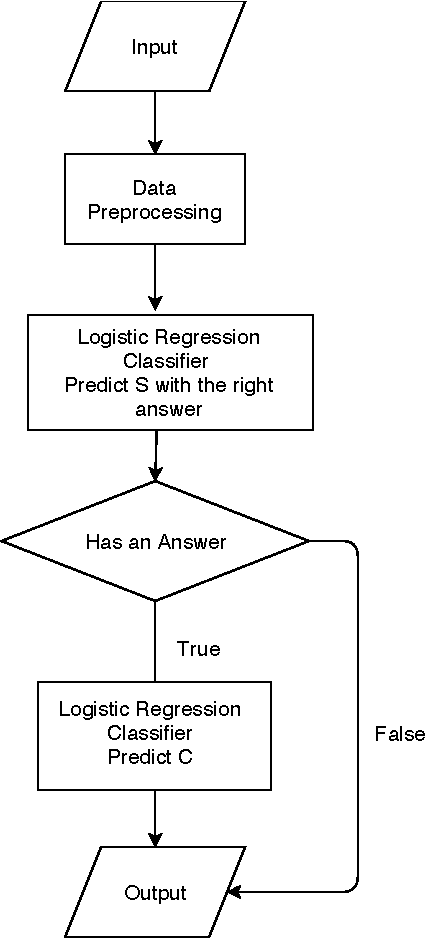
\includegraphics[scale=1]{../Figures/Flowchart.pdf}\centering
  \caption{Flowchart illustrating the two-stage classification approach}
  \label{fig:arc-flowchart}
\end{figure}


\subsection{Feature Extraction} 
% In order for the classifier to find the sentence containing the answer, it must determine the sentence that is most similar to the question, and by similar we mean that a good candidate sentence  1) shares more words with the question. 2) has high cosine similarity with the question. 3) shares a syntactic similarity with the question. Thus, three main features have been selected to this end:
\begin{itemize}
\item \textbf{Cosine Similarity}: for every sentence in the paragraph as well as the question a word vector representation is created via InferSent \citep{ConneauKSBB17}, which is a pre-trained sentence embeddings method that provides semantic representations for English sentences. InferSent is an encoder based on a bi-directional LSTM architecture with max pooling, trained on the Stanford Natural Language Inference (SNLI) dataset. Cosine distance score is calculated for each sentence-question pair. 
\item \textbf{Word Overlap}: calculates the Jaccard score between each sentence-question pair. Jaccard index is a method of computing the explicit similarity between two sets as follows: 
$$
J(Q,S) = \frac{|Q \cap S|}{|Q \cup S|}
$$
where Q and S are sets of words in question and sentence respectively.

\item \textbf{POS Overlap}: computes the Jaccard score over the part-of-speech-tag representation of sentences. In other words, instead of the word tokens, it checks similarity over POS tokens. We use the default POS-tagger in the SpaCy library of Python programming language to obtain the POS representation for the sentences and questions alike.
\end{itemize}
Using the three features above, every question-sentence pair will have three scores and an additional binary feature indicating whether or not the question is answerable. 

\subsection{Training and Result} 
 We get the results shown in \ref{tb:stg1_lr}. Numbers in the class column represents the index of the sentence in the paragraph containing the answer, and -1 indicates that the question has no answer in the paragraph. We also limit the number of sentences to 10. The results show that with simple features, we get an F1 score of 0.71.

\begin{figure}
  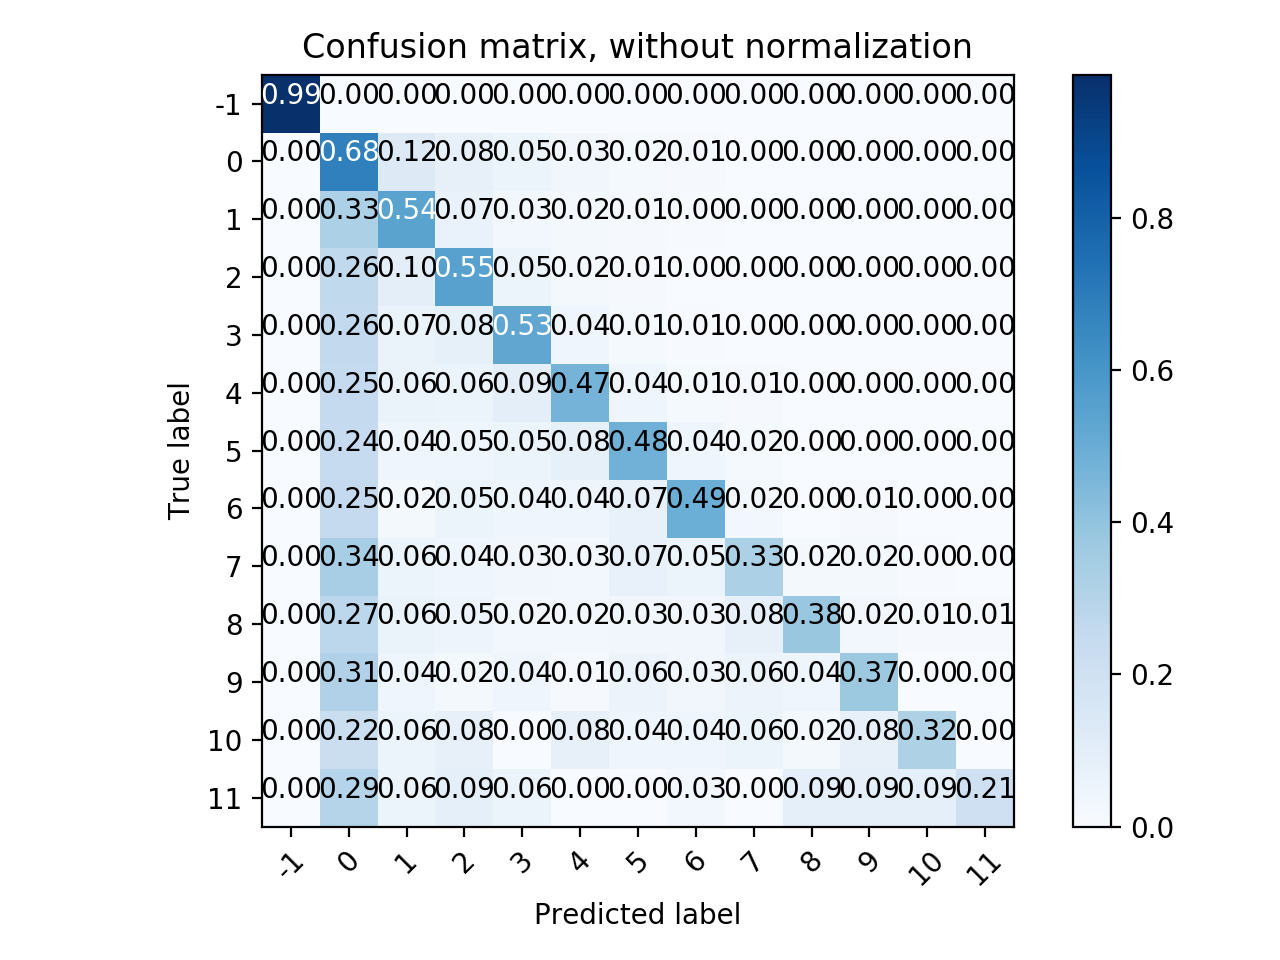
\includegraphics[scale=1]{Figure_1.png}\centering
  \caption{Confusion matrix shows which classes were predicted correctly in Stage One}
  \label{arc_stg1}
\end{figure}

\begin{table}
\centering
\caption{This table shows the results of running a multinomial regularized logistic regression. The class column represents the index of sentences within the paragraph, and -1 represents the unanswerable question case. Unpredicted classes are removed.}
\label{mlr-stage1}
\begin{tabular}{|l|l|l|l|} 
\hline
 \textbf{class}  & \textbf{precision}  & \textbf{recall}  & \textbf{F1-score}   \\ 
\hline
-1               & 1                   & 0.99             & 0.99                \\ 
\hline
0                & 0.47                & 0.68             & 0.56                \\ 
\hline
1                & 0.63                & 0.54             & 0.58                \\ 
\hline
2                & 0.62                & 0.55             & 0.58                \\ 
\hline
3                & 0.62                & 0.53             & 0.57                \\ 
\hline
4                & 0.58                & 0.47             & 0.52                \\ 
\hline
5                & 0.57                & 0.48             & 0.52                \\ 
\hline
6                & 0.57                & 0.49             & 0.53                \\ 
\cline{1-3}
7                & 0.46                & 0.33             & 0.38                \\ 
\hline
8                & 0.56                & 0.38             & 0.45                \\ 
\hline
9                & 0.46                & 0.37             & 0.41                \\ 
\hline
10               & 0.48                & 0.32             & 0.39                \\ 
\hline
11               & 0.35                & 0.21             & 0.26                \\ 
\hline
avg / total      & 0.72                & 0.71             & 0.71                \\
\hline
\end{tabular}
\label{tb:stg1_lr}
\end{table}

\newpage

\section{Stage Two: Predicting the Answer Span}

To select the most plausible answer span from the candidate sentence, we design a number of features, some of which are based on constituent analysis. A constituency parser is used to analyze a sentence into its constituent phrases. For example, the sentence "The quick brown fox jumps over the lazy dog." has the following syntactic (constituency) tree:

\begin{figure}[hbtp]
\centering
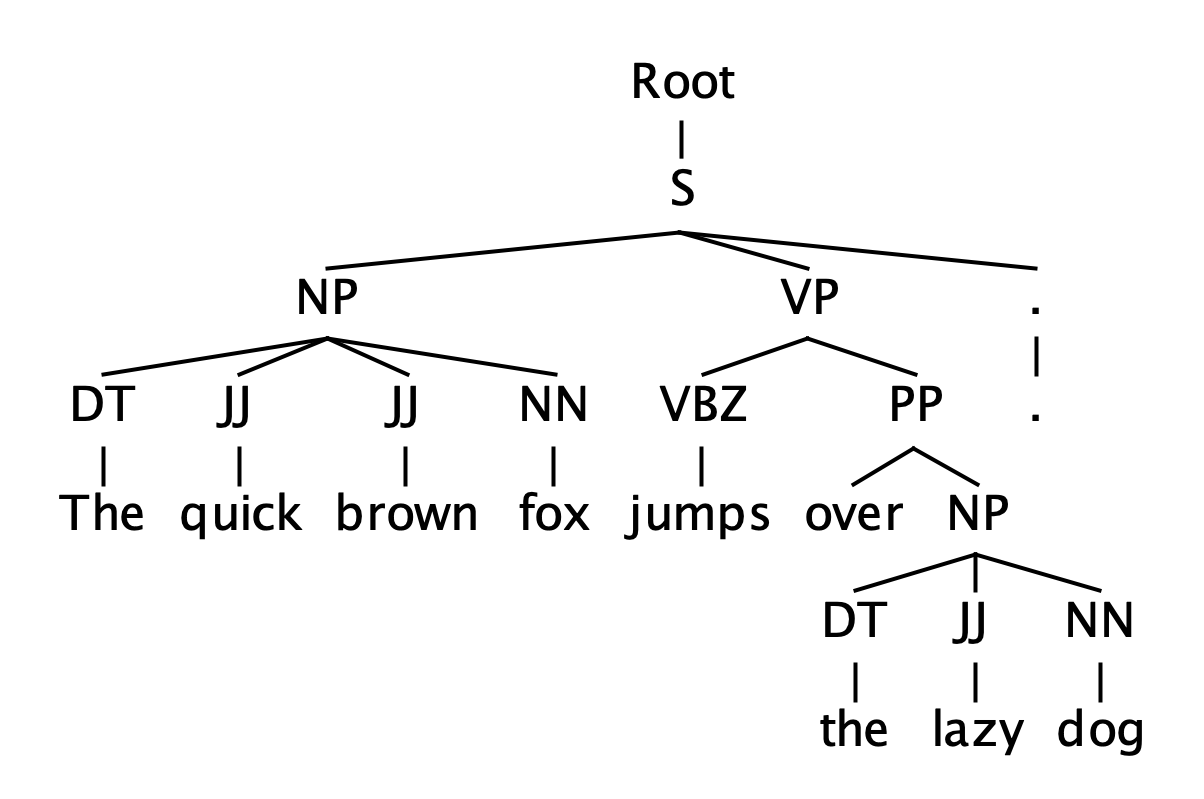
\includegraphics[scale=.2]{../Figures/syntax_tree_example.png}
\caption{Example of Constituency Parse Tree}
\label{fig:parsetree}
\end{figure}



The intuition is an answer span is one of constituents of the best candidate sentence. We use a constituency parser \citep{Kitaev2018} to obtain all constituents in a candidate sentence. These constituents will be the classes from which we pick the right span. For example, the sentence in \ref{fig:parsetree} has the following classes: NP, the quick brown fox; VP, jumps over the lazy dog; VBZ, jumps; PP, over the lazy dog; and NP, the lazy dog. More generally, we design the following features for this stage:

\begin{itemize}
\item \textbf{Contextual Overlap}: Constituents sharing context with the original question are potential candidates to be the correct answers. So we measure the cosine similarity between each constituent and the question:

$${ similarity } = \frac { \sum _ { i = 1 } ^ { n } C _ { |w| } Q _ { i } } { \sqrt { \sum _ { i = 1 } ^ { n } C _ { |w| } ^ { 2 } } \sqrt { \sum _ { i = 1 } ^ { n } Q _ { i } ^ { 2 } } }$$ 

where w is the number of slide window around the candidate constituent. For our purposes features of size 2 and 3 are used.


\item \textbf{Constituent Label}: Constituency parse tree label of the span is combined with wh-word. For example, for the question "Who designed the iPhone prototype?", and its answer "Steve Jobs designed the first prototype for the iPhone.", a constituent label feature is {who-NP, who-V, who-VP, who-PP, etc}. 
\item \textbf{Distributional Distance}: We measure the distributional cosine similarity between the sum of all words in the contextual window and the question using Glove \citep{pennington2014glove}.
\item \textbf{Matching Word Frequencies}: Sum of the TF-IDF of the words that occur in both the question and the sentence containing the candidate answer.
\item \textbf{Lengths}: Number of words to the left and the right of the span.
\end{itemize}

\section{Experiment and Error Analysis}
In this stage, we have done three different training attempts. 
In the first attempt \ref{fig:confmat_stg2a}, we used only two features "contextual overlap" and "constituent label". We also limited the number of classes (constituents) to 30. Using the same training settings and configurations from stage one, the logistic regression achieves a 0.25 F1 score. The confusion matrix shows a clear case of data imbalance. Classes at the beginning have more supporting points, and therefore fewer errors the others. However, our analysis of the errors indicates the wrong answers are partially correct most of the times. Class 2 was identified as class 1 34\% of the time. For example, the answer to the question \emph{At what age did Beyonce meet LaTavia Robertson? }is predicted as \emph{At age eight} when the correct answer is \emph{age eight}. Similarly, class 12 is predicted as class eleven 16\%. The answer to the question \emph{Who supervised the design and implementation of the iPod user interface?} is \emph{Steve Jobs}, but it is predicted as \emph{Of Steve Jobs}. Clearly, the predicted answers are not very far from the true ones. A harsher assumption such as keeping only Noun Phrase constituents could have resolved some of these issues, but we will leave this for future studies. 

\begin{figure}[hbtp]
\begin{subfigure}{\textwidth}
        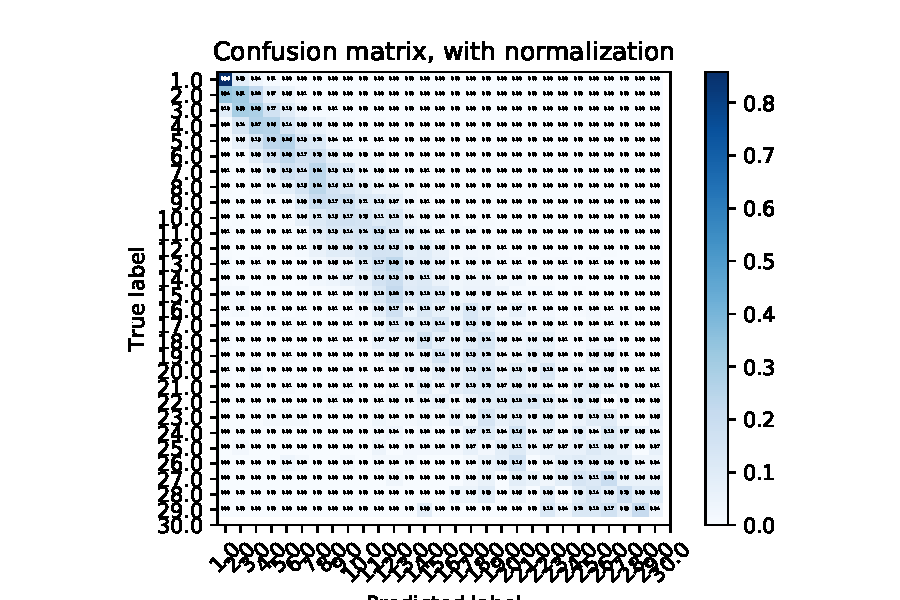
\includegraphics[width=\textwidth]{../Figures/confmat_stg2a.pdf}
        \caption{Confusion Matrix Illustrating the Prediction of Answer Span - First Attempt}
        \label{fig:confmat_stg2a}
    \end{subfigure}
    
    \begin{subfigure}{\textwidth}
        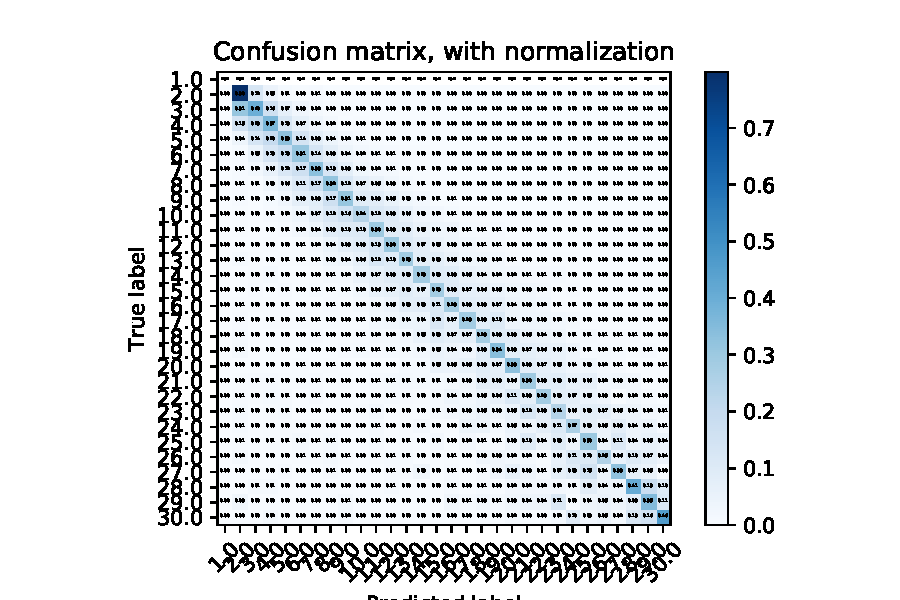
\includegraphics[width=\textwidth]{../Figures/confmat_stg2b.pdf}
        \caption{Confusion Matrix Illustrating the Prediction of Answer Span - Second Attempt}
        \label{fig:confmat_stg2b}
    \end{subfigure}
\end{figure}

Other types of errors are due to literal word matching between the questions and phrases. For example, the answer to the question \emph{How much was public expenditure on the island in 2001-2002?} is predicted to be \emph{Public expenditure} when the true answer is \emph{£10 million}. In this case, the phrase \emph{public expenditure} appears in the question, which makes it a stronger candidate given the features designed. Another example is the answer to \textit{What roles were women recruited for in the 1950s?} is \emph{in medicine, communication}, but it is predicted as \emph{logistics, and administration}. Given the features we have designed, it is very difficult for the classifier to recognize this subtle difference between the classes. 
In the second attempt \ref{fig:confmat_stg2b}, we have added the three remaining features: Distributional Distance, Matching Word Frequencies, and Length, while keeping the same parameters from the first attempt, resulting in an F1 score of 0.35. Looking at the confusion matrices of the first and second attempts, it is apparent that the new features do greatly improve the performance.

In our last experiment, we replaced logistic regression classifier in the second attempt with a 3-layer, feed-forward neural network of 128, 64 and 32 nodes respectively, optimized by Adam optimizer on a 100 epochs . The neural network achieves an F1 score of 0.42. Using a neural network does indeed increases the performance, but its use is not very practical given its configuration. Each node in this neural network is equivalent to one logistic regression classifier, so using a feed-forward neural network with a total of 224 nodes is equal in computational power to 224 logistic regression. 

\section{Future Studies and Recommendations}
Looking at errors produced during the three attempts, we can improve the performance by injecting more linguistic information from Named Entity Recognizers, Semantic Role Labelers, and Dependency Parsers. A Named Entity Recognizer can help answer questions about locations, persons or entities (where, who and which questions). Information derived from a dependency parser and a semantic role labeler can, for example, help resolve cases when the answers are the subjects or the objects of the sentences. Another solution to investigate is to eliminate all constituents, but NP. This idea comes from the assumption that the majority of answers to Wh-questions in SQUAD 2.0 dataset are Noun Phrases. This assumption can help reduce the number of classes to be predicted, so there will be no need to limit the number of outputs to a certain number as we did.

\section{Conclusion}
We introduced a two-step classification method for automatic reading comprehension via the SQUAD 2.0 dataset. Our stage one classifier managed to find whether or not a question is answerable within a given passage and find the sentence containing the right answer with an F1 score of 0.71. Our stage 2 classifier manages to detect the exact span with an F1 score of 0.35 even though the predicted answer is not distant from the exact answer. In order to improve the performance of our approach, future studies should investigate the usefulness of features generated from Named Entity Recognition, Semantic Role Labeling and Dependency Parsing processes, which are expected to be potential solutions to the problems encountered in this research.

%\subsection{First Attempt}
%To select the most plausible answer span from the candidate sentence, we design a number of features:
%\begin{itemize}
%\item \textbf{Constituents}: Using a constituency parser \citep{kitaev2018constituency}, we obtain all constituents in a candidate sentence. These constituents will be the classes from which we pick the right span.
%\item \textbf{Contextual Overlap}: Constituents sharing context with the original question are potential candidates to be the correct answers. So we measure the cosine similarity between each constituent and the question:
%$${ similarity } = \frac { \sum _ { i = 1 } ^ { n } C _ { |w| } Q _ { i } } { \sqrt { \sum _ { i = 1 } ^ { n } C _ { |w| } ^ { 2 } } \sqrt { \sum _ { i = 1 } ^ { n } Q _ { i } ^ { 2 } } }$$ 
%where $w$ is the number of slide window around the candidate constituent. For our purposes features of size 2 and 3 are used. 
%
%\item \textbf{Constituent Label}: Constituency parse tree label of the span combined with wh-word.
%\end{itemize}
%Out of 85K training example, the answer spans of nearly half of them are not within the constituents. However, answers can be part of the constituents.  For example, an answer span might be \textit{L'official} and the nearest constituent is \textit{L'official Magazine}. So for our first attempt, we remove all data points whose answers are not explicitly found within the constituents. This results in around 45K data point. Next, we train a logistic regression classifier with L2 regularization and 100 epochs, optimized by newton method 'newton-cg' on a MacBook Pro laptop with core i5 processor and 8 GB of RAM. Python modules used are Scikit-learn and SpaCy. The latter is used to drive the attentive-neural constituency parser (Kitaev, 2018). The result is 0.25 F1 score.
%
%
%
%
%\subsection{Error Analysis of First Attempt}
%%\subsection{Format of Electronic Manuscript}
%%\label{sect:pdf}
%
%\begin{figure}
%  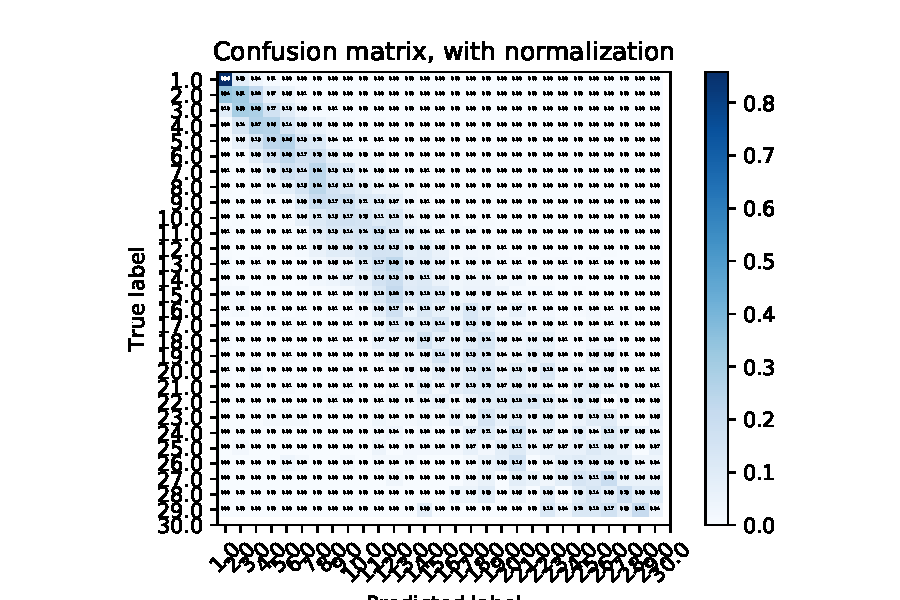
\includegraphics[scale=1]{../Figures/fig_iter1.pdf} \centering
%  \caption{Confusion Matrix illustrating the first iteration of Stage2 LR. }
%\end{figure} 
%
%
%
%Looking at the confusion matrix, we notice that there is a data imbalance. Classes at the beginning have more supporting points, and therefore have less error than the others. However, class 2 has been identified as class 1 34\%. For example, the answer of \textit{At what age did Beyonce meet LaTavia Robertson?} is predicted as \textit{At age eight} while the correct answer is \textit{age eight}. Another example, the answer for \textit{How much was public expenditure on the island in 2001-2002?} is predicted to be \textit{Public expenditure} while the true answer is \textit{£10 million}. In this case, the phrase public expenditure appears in the question, which is a stronger candidate given the features designed.
%Similarly, class 12 is predicted as class eleven 16\%. For example, the answer to the question \textit{Who supervised the design and implementation of the iPod user interface?} is \textit{Steve Jobs}, but it is predicted as \textit{Of Steve Jobs}. Another example, answer to \textit{What roles were women recruited for in the 1950s?} is \textit{in medicine, communication}, but it is predicted as \textit{logistics, and administration}. Given the features, we have designed it is very difficult for the classifier to recognize this settle difference between the classes. 
%
%
%\subsection{Second Attempt}
%
%In the first attempt, we have sacrificed valuable data because the answer span was not within the constituents of the candidate sentence. This time, we use all 85K, but we will face the same problem introduced in the previous section. The answer span can be a member of more than one constituent in the same sentence, and this will impose a very hard constraint on the performance because the inference can be close but not exact. Also because this problem requires more feature engineering efforts, we decided to leave it for future studies. Instead, we will set the target to the first constituent of which the span is a member. However, we will add three more features:
%
%\begin{itemize}
%\item \textbf{Distributional Distance}: We measure the distributional cosine similarity between the sum of all words in the contextual window and the question using Glove (Pennington, 2012). 
%
%\item \textbf{Matching Word Frequencies}: Sum of the TF-IDF of the words that occur in both the question and the sentence containing the candidate answer.
%
%\item \textbf{Lengths}: Number of words to the left and the right of the span.
%\end{itemize}
%
%For classification, we compare the performance of a logistic regression classifier with a similar configuration as the first stage to 3-layer feed-forward neural network of 128, 64 and 32 nodes respectively. The logistic regression achieves 0.35 F1 while the neural network does 0.42 F1 using Adam optimizer and 100 epochs. Looking at the confusion matrix, it is apparent that the new features (tf-idf and distributional cosine similarity) improve the performance. However, they could not recognize the settle difference among the phrase.  \\
%
%
%\begin{figure}
%  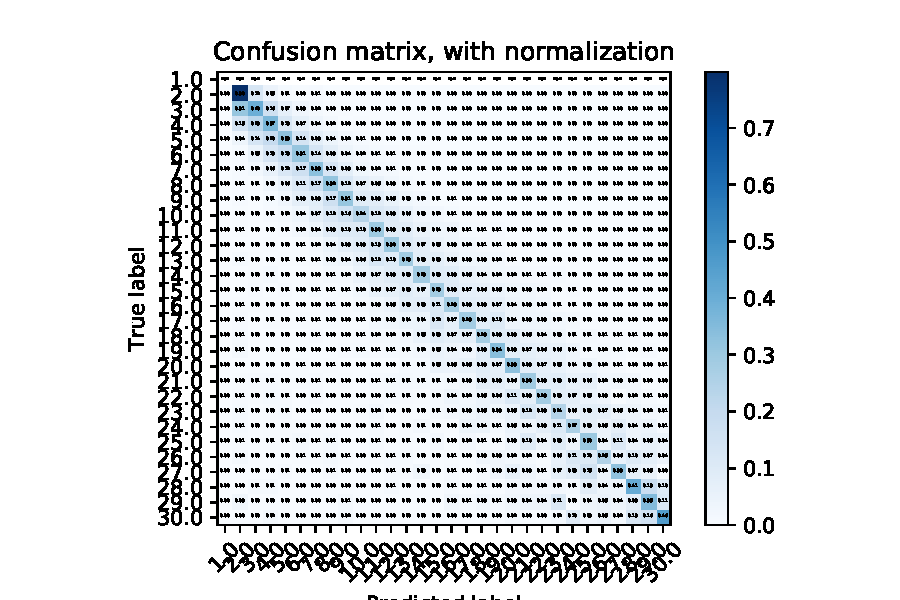
\includegraphics[scale=1]{../Figures/fig_1.pdf} 
%  \caption{Confusion Matrix illustrating the Second iteration of Stage2 LR. }
%\end{figure} 
%
%
%\section{Conclusion}
%
%We introduced a two-step classification method for automatic reading comprehension via SQUAD 2.0 dataset. Our stage1 classifier managed to find whether or not a question is answerable within a given passage and find the sentence containing the right answer with F1 score of 0.71. Our stage2 classifier manages to detect the exact span with F1 score of 0.35 even though the predicted answer is not distant from the exact answer. In order to improve the performance of our approach, future studies should investigate the usefulness of features generated from Named Entity Recognition, Semantic Role Labeling and Dependency Parsing processes, which are expected to be potential solutions to the problems we faced in this work. 